\documentclass[border=5pt, multi, tikz]{standalone}
\usepackage{import}
\usepackage{amsmath}
\usepackage{amssymb}
\usetikzlibrary{positioning, arrows.meta, shapes.geometric, calc, fit, backgrounds}

% 定义颜色
\definecolor{transformercolor}{RGB}{147, 112, 219}
\definecolor{tcncolor}{RGB}{255, 140, 0}
\definecolor{fusioncolor}{RGB}{70, 130, 180}
\definecolor{inputcolor}{RGB}{100, 149, 237}
\definecolor{outputcolor}{RGB}{60, 179, 113}

\begin{document}
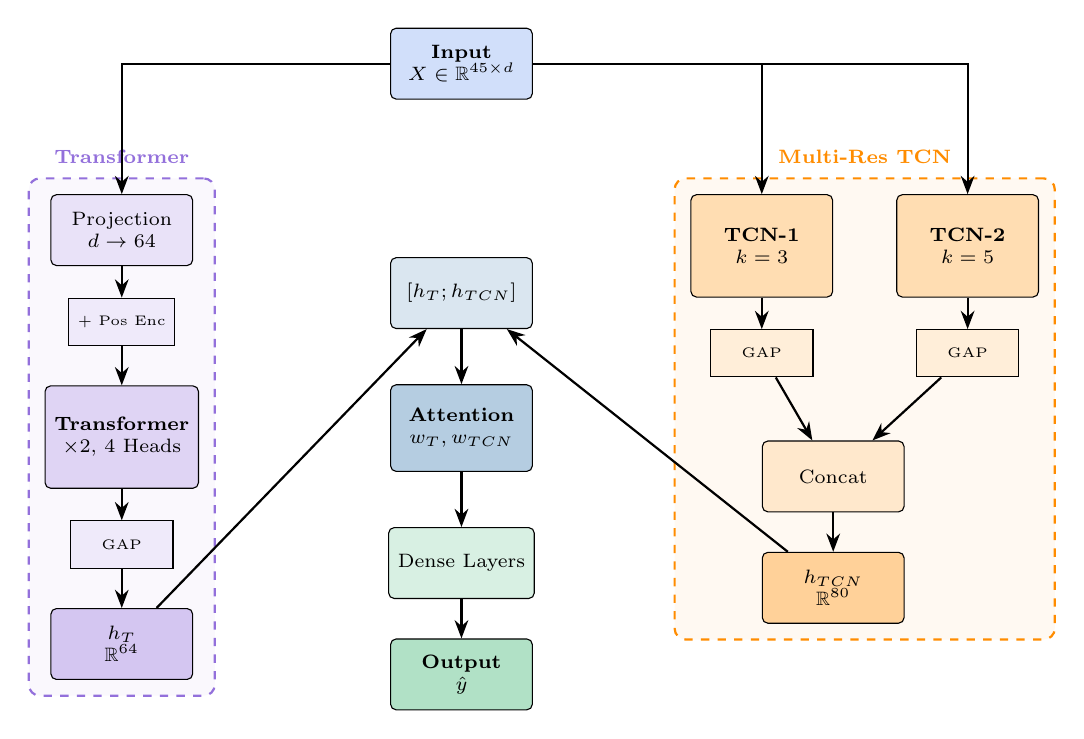
\begin{tikzpicture}[
    node distance=0.6cm and 1.5cm,
    box/.style={rectangle, draw, minimum width=1.8cm, minimum height=0.9cm, align=center, font=\scriptsize, rounded corners=2pt},
    smallbox/.style={rectangle, draw, minimum width=1.3cm, minimum height=0.6cm, align=center, font=\tiny},
    arrow/.style={-Stealth, thick},
    bigarrow/.style={-Stealth, ultra thick},
    dashedarrow/.style={-Stealth, thick, dashed},
]

% ============ 输入 ============
\node[box, fill=inputcolor!30] (input) 
      {\textbf{Input}\\$X \in \mathbb{R}^{45 \times d}$};

% ============ 分支 ============
% Transformer Branch (Left)
\node[box, fill=transformercolor!20, below left=1.2cm and 2.5cm of input] (trans_proj) 
      {Projection\\$d \rightarrow 64$};
      
\node[smallbox, fill=transformercolor!15, below=0.4cm of trans_proj] (pos) 
      {+ Pos Enc};
      
\node[box, fill=transformercolor!30, below=0.5cm of pos, minimum height=1.3cm] (transformer) 
      {\textbf{Transformer}\\$\times 2$, 4 Heads};
      
\node[smallbox, fill=transformercolor!15, below=0.4cm of transformer] (trans_gap) 
      {GAP};
      
\node[box, fill=transformercolor!40, below=0.5cm of trans_gap] (trans_out) 
      {$h_T$\\$\mathbb{R}^{64}$};

% TCN Branch (Right)
\node[box, fill=tcncolor!30, below right=1.2cm and 2cm of input, minimum height=1.3cm] (tcn1) 
      {\textbf{TCN-1}\\$k=3$};
      
\node[box, fill=tcncolor!30, right=0.8cm of tcn1, minimum height=1.3cm] (tcn2) 
      {\textbf{TCN-2}\\$k=5$};

\node[smallbox, fill=tcncolor!15, below=0.4cm of tcn1] (gap1) {GAP};
\node[smallbox, fill=tcncolor!15, below=0.4cm of tcn2] (gap2) {GAP};

\node[box, fill=tcncolor!20, below=0.8cm of gap1.south-|tcn1.south east] (concat) 
      {Concat};

\node[box, fill=tcncolor!40, below=0.5cm of concat] (tcn_out) 
      {$h_{TCN}$\\$\mathbb{R}^{80}$};

% ============ 融合层 ============
\node[box, fill=fusioncolor!20, below=2cm of input] (fusion_concat) 
      {$[h_T; h_{TCN}]$};

\node[box, fill=fusioncolor!40, below=0.7cm of fusion_concat, minimum height=1.1cm] (attention) 
      {\textbf{Attention}\\$w_T, w_{TCN}$};

% ============ 预测头 ============
\node[box, fill=outputcolor!20, below=0.7cm of attention] (pred_head) 
      {Dense Layers};
      
\node[box, fill=outputcolor!40, below=0.5cm of pred_head] (output) 
      {\textbf{Output}\\$\hat{y}$};

% ============ 箭头 ============
% Input分支
\draw[arrow] (input) -| (trans_proj);
\draw[arrow] (input) -| (tcn1);
\draw[arrow] (input) -| (tcn2);

% Transformer流
\draw[arrow] (trans_proj) -- (pos);
\draw[arrow] (pos) -- (transformer);
\draw[arrow] (transformer) -- (trans_gap);
\draw[arrow] (trans_gap) -- (trans_out);

% TCN流
\draw[arrow] (tcn1) -- (gap1);
\draw[arrow] (tcn2) -- (gap2);
\draw[arrow] (gap1) -- (concat);
\draw[arrow] (gap2) -- (concat);
\draw[arrow] (concat) -- (tcn_out);

% 融合
\draw[arrow] (trans_out) -- (fusion_concat);
\draw[arrow] (tcn_out) -- (fusion_concat);
\draw[arrow] (fusion_concat) -- (attention);

% 输出
\draw[arrow] (attention) -- (pred_head);
\draw[arrow] (pred_head) -- (output);

% ============ 背景框 ============
\begin{pgfonlayer}{background}
    \node[draw=transformercolor, thick, dashed, rounded corners, fit={(trans_proj) (transformer) (trans_out)}, 
          fill=transformercolor!5, inner sep=0.2cm] (trans_box) {};
    \node[above=0.05cm of trans_box, font=\scriptsize\bfseries, text=transformercolor] {Transformer};
    
    \node[draw=tcncolor, thick, dashed, rounded corners, fit={(tcn1) (tcn2) (tcn_out)}, 
          fill=tcncolor!5, inner sep=0.2cm] (tcn_box) {};
    \node[above=0.05cm of tcn_box, font=\scriptsize\bfseries, text=tcncolor] {Multi-Res TCN};
\end{pgfonlayer}

\end{tikzpicture}
\end{document}
